\documentclass[11pt, letterpaper]{article}

% ---------- packages ----------
\usepackage[margin=0.7in]{geometry}
\usepackage{tcolorbox}
\usepackage{enumitem}
\usepackage{hyperref}
\usepackage{xcolor}
\usepackage{titlesec}
\usepackage{fancyhdr}
\usepackage{graphicx}
\usepackage{tabularx}
\usepackage{booktabs}

% ---------- colors ----------
\definecolor{boxborder}{RGB}{60, 90, 150}
\definecolor{boxbg}{RGB}{245, 248, 255}
\definecolor{headcolor}{HTML}{00636f}
\definecolor{placeholder}{RGB}{140, 140, 140}

% ---------- tcolorbox style ----------
\tcbset{
  sectionbox/.style={
    colframe=boxborder,
    colback=boxbg,
    boxrule=0.6pt,
    arc=2pt,
    left=6pt, right=6pt, top=4pt, bottom=4pt,
    fontupper=\scriptsize,
  }
}

% ---------- placeholder command ----------
\newcommand{\placeholder}[1]{\textcolor{placeholder}{\textit{#1}}}

% ---------- section formatting ----------
\titleformat{\section}
  {\normalsize\bfseries\color{headcolor}}{\thesection.}{0.4em}{}
\titlespacing*{\section}{0pt}{6pt}{2pt}

% ---------- header / footer ----------
\pagestyle{fancy}
\fancyhf{}
\renewcommand{\headrulewidth}{0.4pt}
\lhead{\small\color{headcolor} CS 4100 -- Project Executive Summary}
%\rhead{\small\color{headcolor} Semester, Year}
\cfoot{\small\thepage}

% ---------- suppress paragraph indent ----------
\setlength{\parindent}{0pt}
\setlength{\parskip}{3pt}

\begin{document}

% ===== TITLE BLOCK =====
\begin{center}
  {\Large\bfseries\color{headcolor} Diet Planner App}\\[4pt]
  {\normalsize Ekrem Karakas, Member 2, Member 3, Member 4}\\[2pt]
\end{center}

\vspace{4pt}

% ===== 1. MOTIVATION & PROBLEM STATEMENT =====
\section{Motivation \& Problem Statement}
\begin{tcolorbox}[sectionbox, height=4.6cm, valign=top]
  % --> REMOVE THE \placeholder ENV BELOW, AND ADD YOUR OWN TEXT  <-- %
  \placeholder{%
    Describe the real-world problem your project addresses and explain
    why it matters. Identify the specific gap, limitation, or
    opportunity that motivates this work. State the core research
    question or engineering goal in one clear sentence.
    Cite relevant prior work or context that frames the problem
    (1--2 references are sufficient). Aim for roughly 8--12 sentences.}

TODO - GOT FROM PROPOSAL MIGHT NEED UPDATING

Balancing all the various micro and macronutrients can be a challenge, with different foods all having different amounts of each. Because there aren’t good ways to ingest just one type of nutrient, it can be difficult to balance your diet such that every daily recommendation is met without going over or under. Many meal-planning tools generate a static daily or weekly plan that assumes the user will follow it exactly. In practice, people often deviate from their plans by eating unplanned meals or snacks, which can lead to nutritional imbalance.
Existing tools like MacroFactor can help by generating “a dynamic nutrition plan that adjusts your diet to fit your metabolism”, but following a strict plan may not be the best option if some nutrients are unplanned, but consumed anyway. A lot of these apps also rely heavily on tracking rather than making recommendations, such as MacroFactor advertising that the app can be used to “track vitamins and minerals, set custom targets, and dive into rich analytics”. While providing this information can be useful, applying machine learning on top of this can generate optimal nutritional feedback dynamically. Hungryroot is another existing tool, a personalized grocery delivery and meal recommendation service designed to simplify healthy eating. When users sign up, they take a quiz about their dietary preferences, nutritional goals, and food dislikes. Based on these inputs, Hungryroot curates a weekly selection of grocery items and simple recipes tailored to the user’s profile. The platform blends grocery delivery with meal suggestions so that users receive ingredients and recipe ideas to match their overall preferences and goals. However, its recommendations are largely static for the week and do not adjust based on what the user actually eats throughout the day.
We propose to build a dynamic meal planning system that updates its recommendations throughout the day based on meals the user manually logs. After each logged meal, the system recalculates remaining nutritional needs and adjusts the plan for the rest of the day to better meet dietary guidelines and user constraints. The goal is to help users make better follow-up choices rather than expecting perfect adherence to an initial plan. To accomplish this we plan on using a matrix based optimization machine learning algorithm such as naive bayes classifier. We plan on training our machine learning model on publicly available nutritional datasets such as this one from Kaggle.
\end{tcolorbox}

% ===== 2. APPROACH =====
\section{Approach}
\begin{tcolorbox}[sectionbox, height=7.0cm, valign=top]
% --> REMOVE THE \placeholder ENV BELOW, AND ADD YOUR OWN TEXT  <-- %
  \placeholder{%
    Summarize your technical approach at a high level. Describe the
    system architecture or methodology, key algorithms or models used,
    and the most important design decisions. If applicable, include a
    small figure or diagram (use \textbackslash includegraphics), and resize to stay within bounded box area.
    Mention the primary tools, frameworks, or libraries
    (e.g., PyTorch, Mesa, Gymnasium, PettingZoo).
    Clearly state any assumptions or scope limitations.
    Aim for roughly 10--15 sentences or equivalent with an optional figure.}

    Preprocessing

    We are pulling data from two sources (USDA Foundation Foods and Open Food Facts). The data is normalized to a per 100g basis, cleaned by dropping incomplete or unrealistic rows, and filtered down to 10,000 foods.

    Simulated Annealing

    The implementation represents a meal as a tuple of (food\_index, multiplier). The meal plan is a list of meals, one per meal slot. The state is initialized using the greedy-init algorithm. At each step, one of three neighbor moves is applied. Replace swaps a slot's food for any food from the dataset. Swap exchanges two foods between their slots. Resize updates a meal's multiplier by a random delta taken from a uniform distribution between -0,5 and 0,5. Each candidate is evaluated using the energy function (1 - fitness function). Better neighboring states are always accepted while worse plans are accepted probabilistically based on the current temperature that decays geometrically by time.

\end{tcolorbox}

% ===== 3. KEY RESULTS =====
\section{Key Results}
\begin{tcolorbox}[sectionbox, height=8cm, valign=top]
% --> REMOVE THE \placeholder ENV BELOW, AND ADD YOUR OWN TEXT  <-- %
  \placeholder{%
    Present the most important quantitative and/or qualitative results.
    Include 1--2 key metrics, comparisons, or summary statistics.
    Interpret the results: what worked well, what was surprising,
    and how do the outcomes compare with your initial expectations
    or baselines? Aim for roughly 8--12 sentences or equivalent. Small tables, figures, or charts may be embedded here, and/or in the first box on the next page (examples on next page).}
\end{tcolorbox}

\newpage

\begin{tcolorbox}[sectionbox, height=8cm, valign=top]
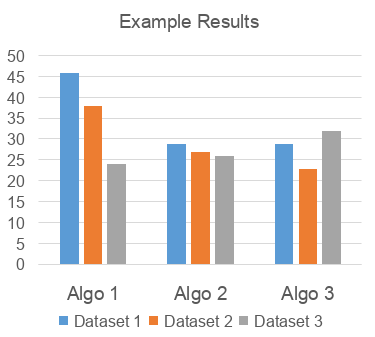
\includegraphics[width=0.42\linewidth]{Picture.png}\hfill
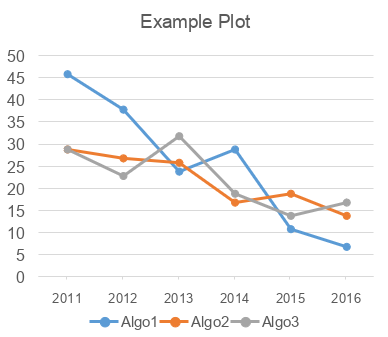
\includegraphics[width=0.42\linewidth]{Picture2.png}
  \\
  % --> REMOVE THE \placeholder ENV BELOW, AND ADD YOUR OWN TEXT  <-- %
  \placeholder{%
  Replace these figures with your own, or remove them and use this space for more text. Ensure all text in your figures are clear and readable at this scale, similar to these examples.
   }
\end{tcolorbox}
% ===== 4. CHALLENGES & LESSONS LEARNED =====
\section{Challenges \& Lessons Learned}
\begin{tcolorbox}[sectionbox, height=4.4cm, valign=top]
% --> REMOVE THE \placeholder ENV BELOW, AND ADD YOUR OWN TEXT  <-- %
  \placeholder{%
    Discuss the main technical and organizational challenges
    encountered during the project. For each challenge, briefly
    explain how the team addressed or mitigated it.
    Highlight lessons learned that would be valuable for future
    work or for other teams tackling similar problems.
    Aim for roughly 8--12 sentences.}
\end{tcolorbox}

% ===== 5. INDIVIDUAL CONTRIBUTIONS =====
\section{Individual Contributions}
\begin{tcolorbox}[sectionbox, height=4.3cm, valign=top]
% --> REMOVE THE \placeholder ENV BELOW BEFORE SUBMISSION  <-- %
  \placeholder{Replace the table below with your team's actual contributions.}

  \vspace{4pt}
  \centering
  \begin{tabularx}{0.95\textwidth}{l X c}
    \toprule
    \textbf{Member} & \textbf{Primary Contributions} & \textbf{Approx.\ \%} \\
    \midrule
    Ekrem Karakas & \placeholder{Preprocessing Data, Simulated Annealing, Energy Function}          & 20\% \\
    Member 2 & \placeholder{e.g., Data pipeline, evaluation scripts}   & 20\% \\
    Member 3 & \placeholder{e.g., Environment design and implementation} & 20\% \\
    Member 4 & \placeholder{e.g., Data pipeline, evaluation scripts}  & 20\% \\
    Member 5 & \placeholder{e.g., System design, agent logic}  & 20\% \\
    \bottomrule
  \end{tabularx}
\end{tcolorbox}

% ===== 6. REPOSITORY & REFERENCES =====
\section{Repository \& References}
\begin{tcolorbox}[sectionbox, height=4.5cm, valign=top]
  \textbf{GitHub Repository:}
  \placeholder{\href{https://github.com/4oore/CS4100-Group-Project}%
       {\texttt{https://github.com/4oore/CS4100-Group-Project}}}\\
    \placeholder{Ensure repo is public, or add instructor as a collaborator.}\vspace{1pt}

  \textbf{Project Tracker:} \placeholder{\href{https://github.com/users/4oore/projects/1}{\texttt{https://github.com/users/4oore/projects/1}}}

  \vspace{6pt}
  \textbf{Key References:}
  \begin{enumerate}[leftmargin=1.4em, itemsep=1pt, topsep=2pt, label={[\arabic*]}]
    \item \placeholder{Author(s), ``Title,'' Venue, Year. Brief annotation.}
    \item \placeholder{Author(s), ``Title,'' Venue, Year. Brief annotation.}
    \item \placeholder{Author(s), ``Title,'' Venue, Year. Brief annotation.}
  \end{enumerate}

  \vspace{4pt}
  \placeholder{Add or remove reference entries as needed (3--4 recommended).}
\end{tcolorbox}

\end{document}
